% Created 2023-01-04 Qua 14:45
% Intended LaTeX compiler: pdflatex
\documentclass[a4paper, 12pt]{article}
\usepackage[utf8]{inputenc}
\usepackage[T1]{fontenc}
\usepackage{graphicx}
\usepackage{longtable}
\usepackage{wrapfig}
\usepackage{rotating}
\usepackage[normalem]{ulem}
\usepackage{amsmath}
\usepackage{amssymb}
\usepackage{capt-of}
\usepackage{hyperref}
\usepackage[margin=0.8in]{geometry}
\setlength{\textheight}{230mm}
\setlength{\textwidth}{160mm}
\setlength{\voffset}{-10mm}
\setlength{\oddsidemargin}{0mm}
\setlength{\evensidemargin}{0mm}
\addtolength{\parskip}{0.33\baselineskip}
\setlength\parindent{24pt}
\author{Davi Raubach Tuchtenhagen}
\date{\today}
\title{(Pré)-composição 2\\\medskip
\large Oficina de Música de Curitiba 2023}
\hypersetup{
 pdfauthor={Davi Raubach Tuchtenhagen},
 pdftitle={(Pré)-composição 2},
 pdfkeywords={},
 pdfsubject={},
 pdfcreator={Emacs 29.0.50 (Org mode 9.5.4)}, 
 pdflang={English}}
\begin{document}

\maketitle

\section*{Estrutura geral}
\label{sec:org6ee895d}
Consegui pensar em três fragmentos de 1 a 1:30 minutos que conectados formam a peça completa.

As imagens abaixo apresentam um percurso dos materiais. O percurso para cada um dos 3 fragmentos está completo neste planejamento e poderia ficar interessante.

\begin{center}
\includegraphics[width=.9\linewidth]{images/20230104_085554.jpg}
\end{center}

\begin{center}
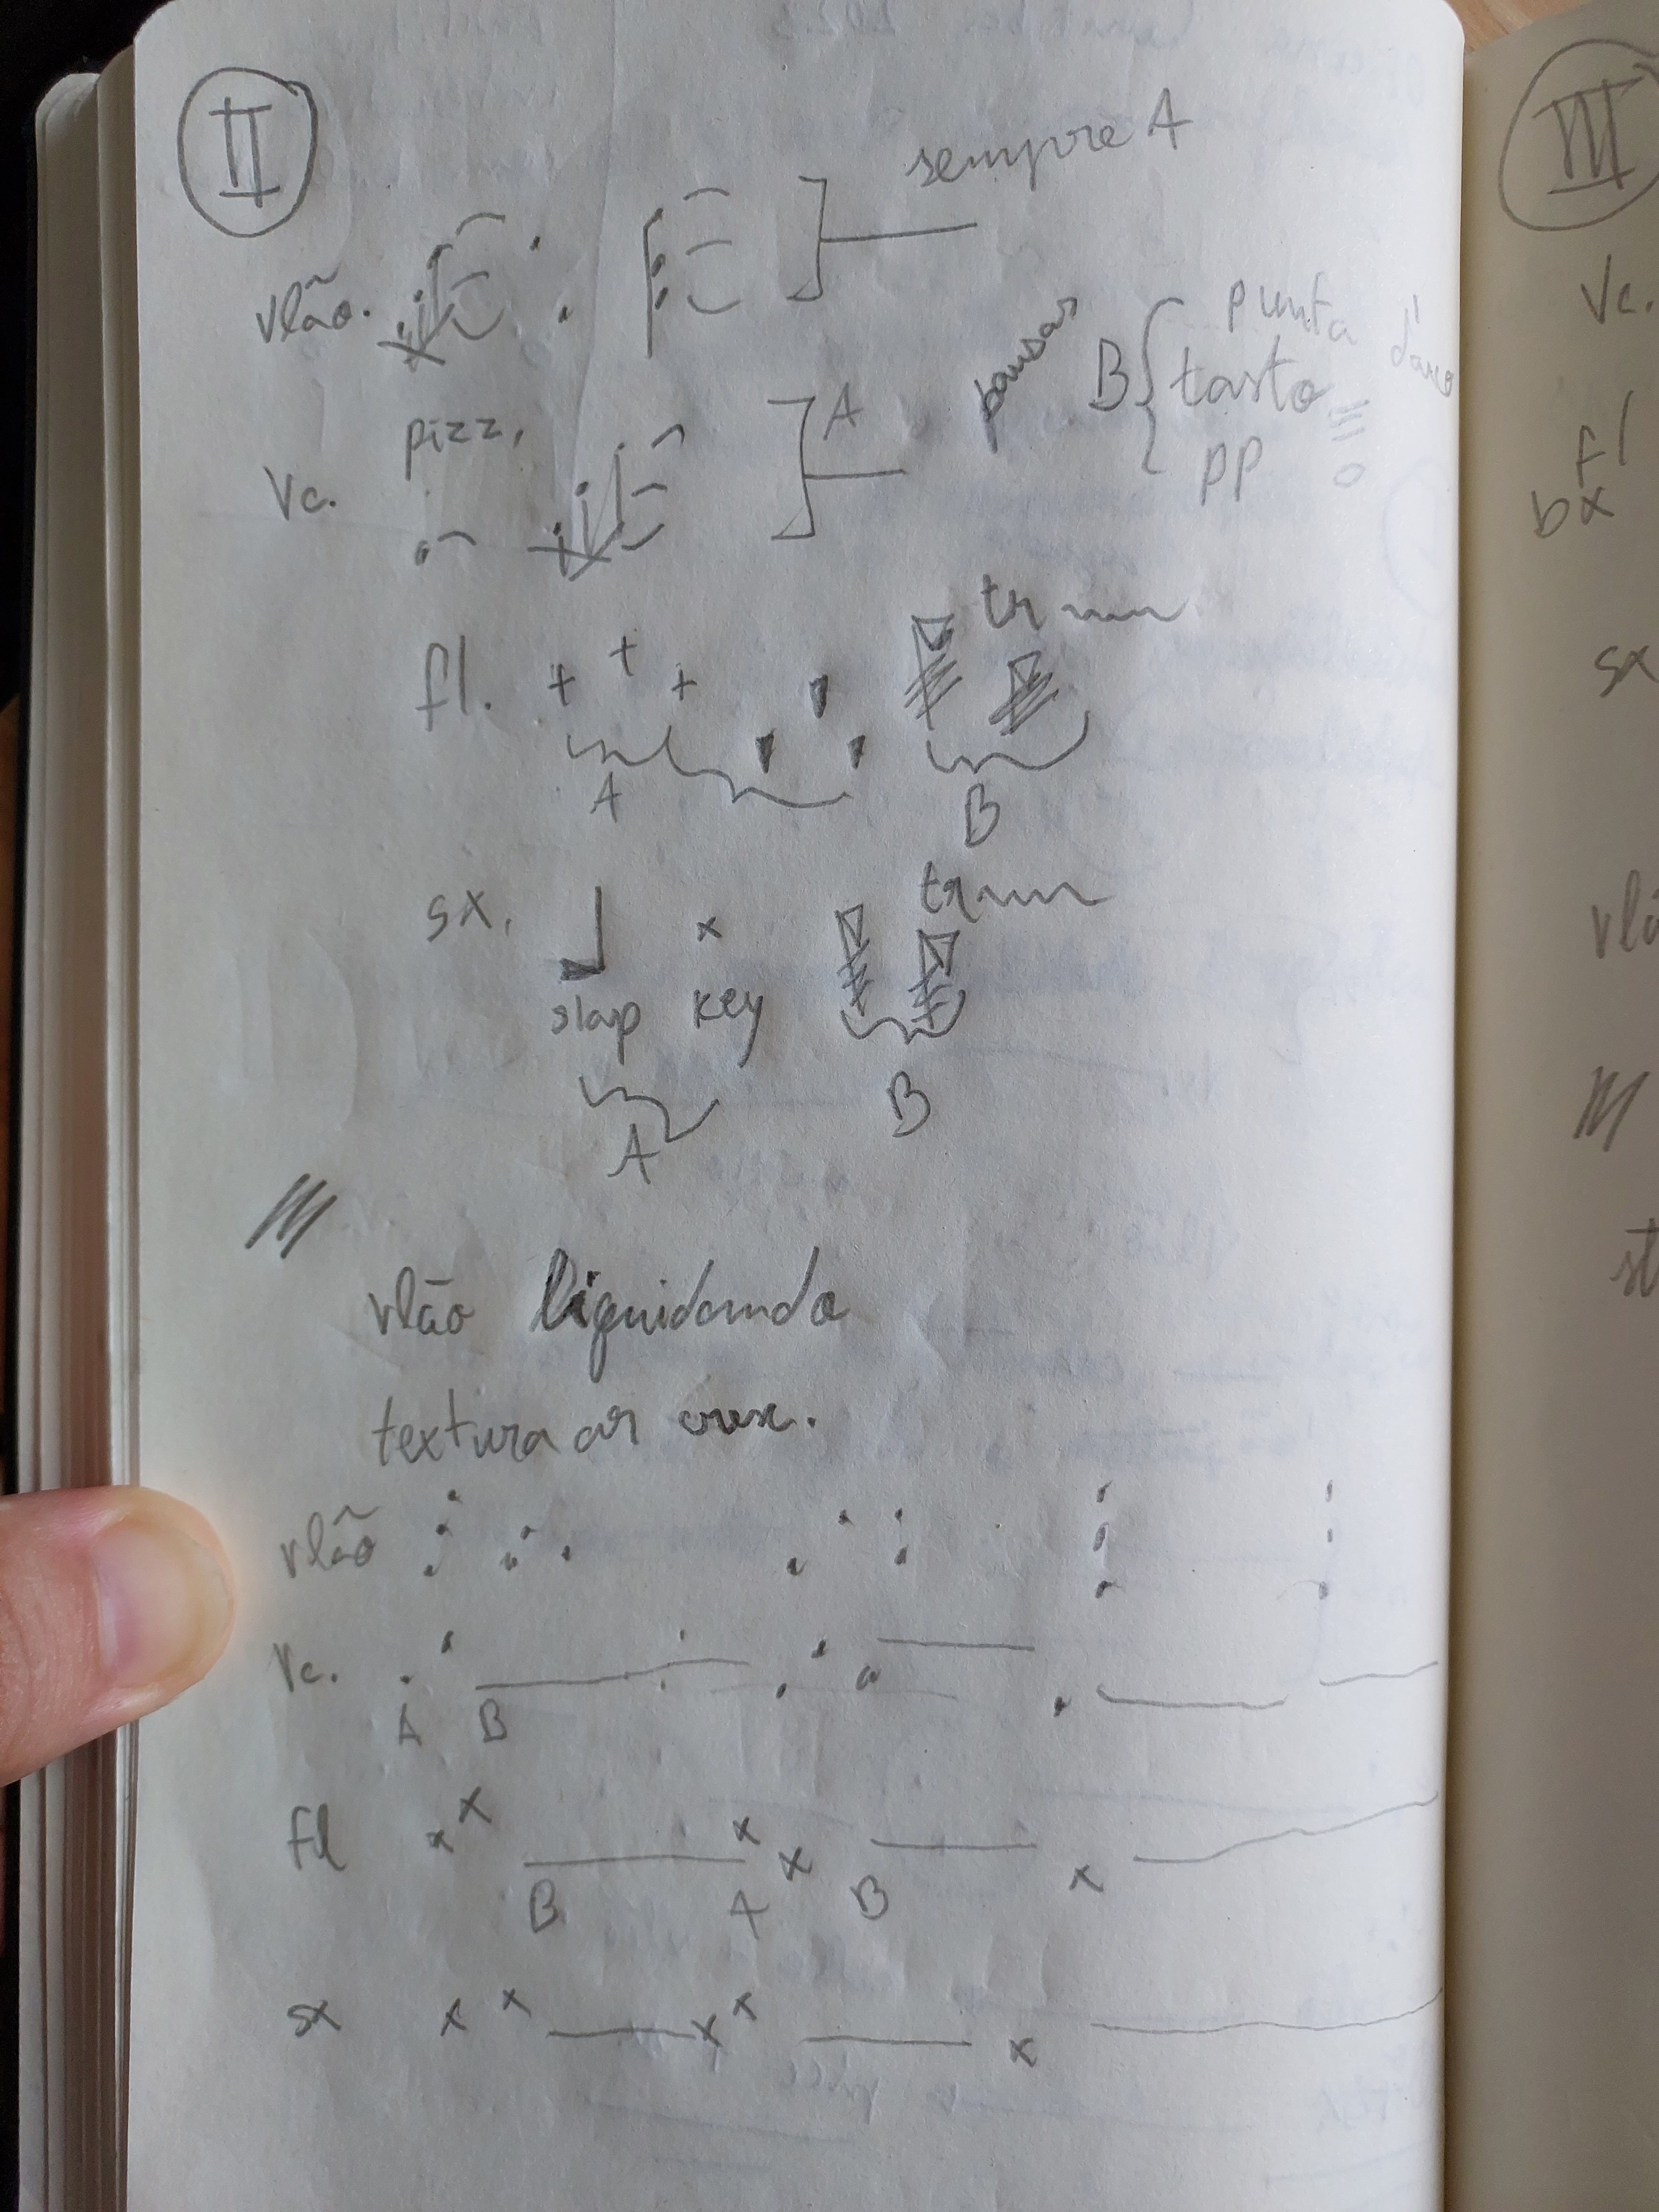
\includegraphics[width=10cm]{images/20230104_085602.jpg}
\end{center}

\begin{center}
\includegraphics[width=10cm]{images/20230104_085609.jpg}
\end{center}

\begin{center}
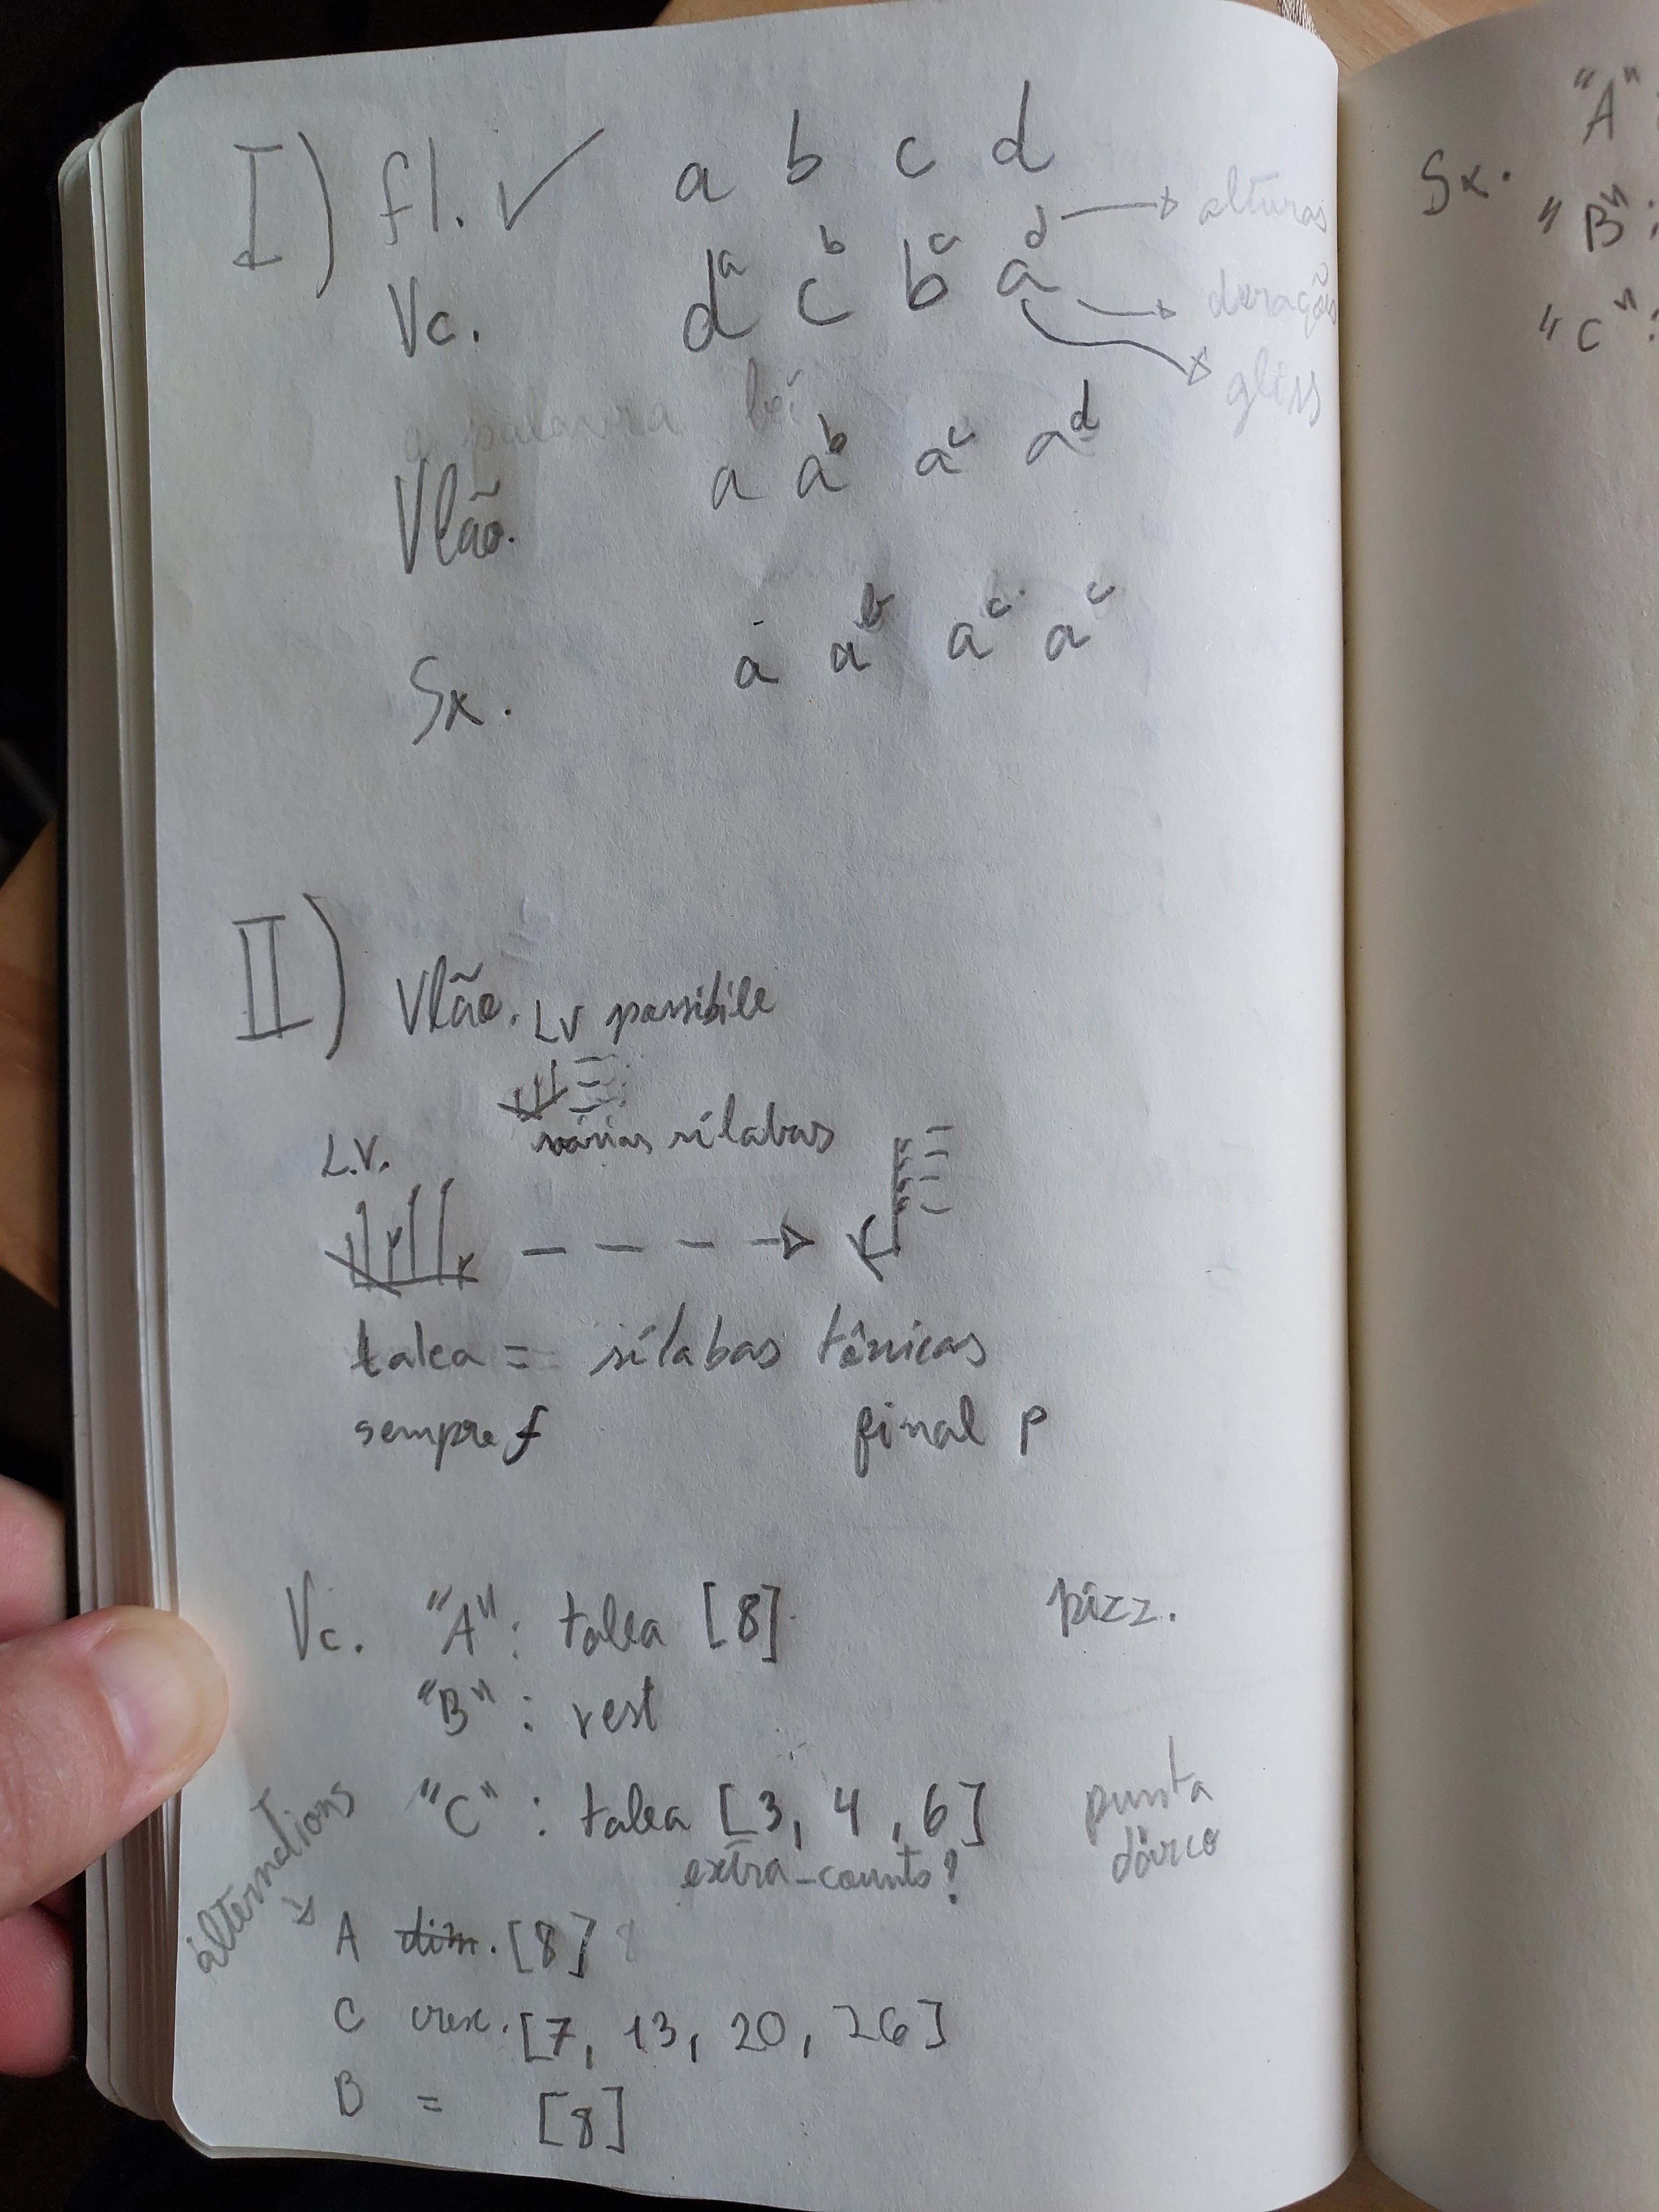
\includegraphics[width=10cm]{images/20230104_085625.jpg}
\end{center}

\begin{center}
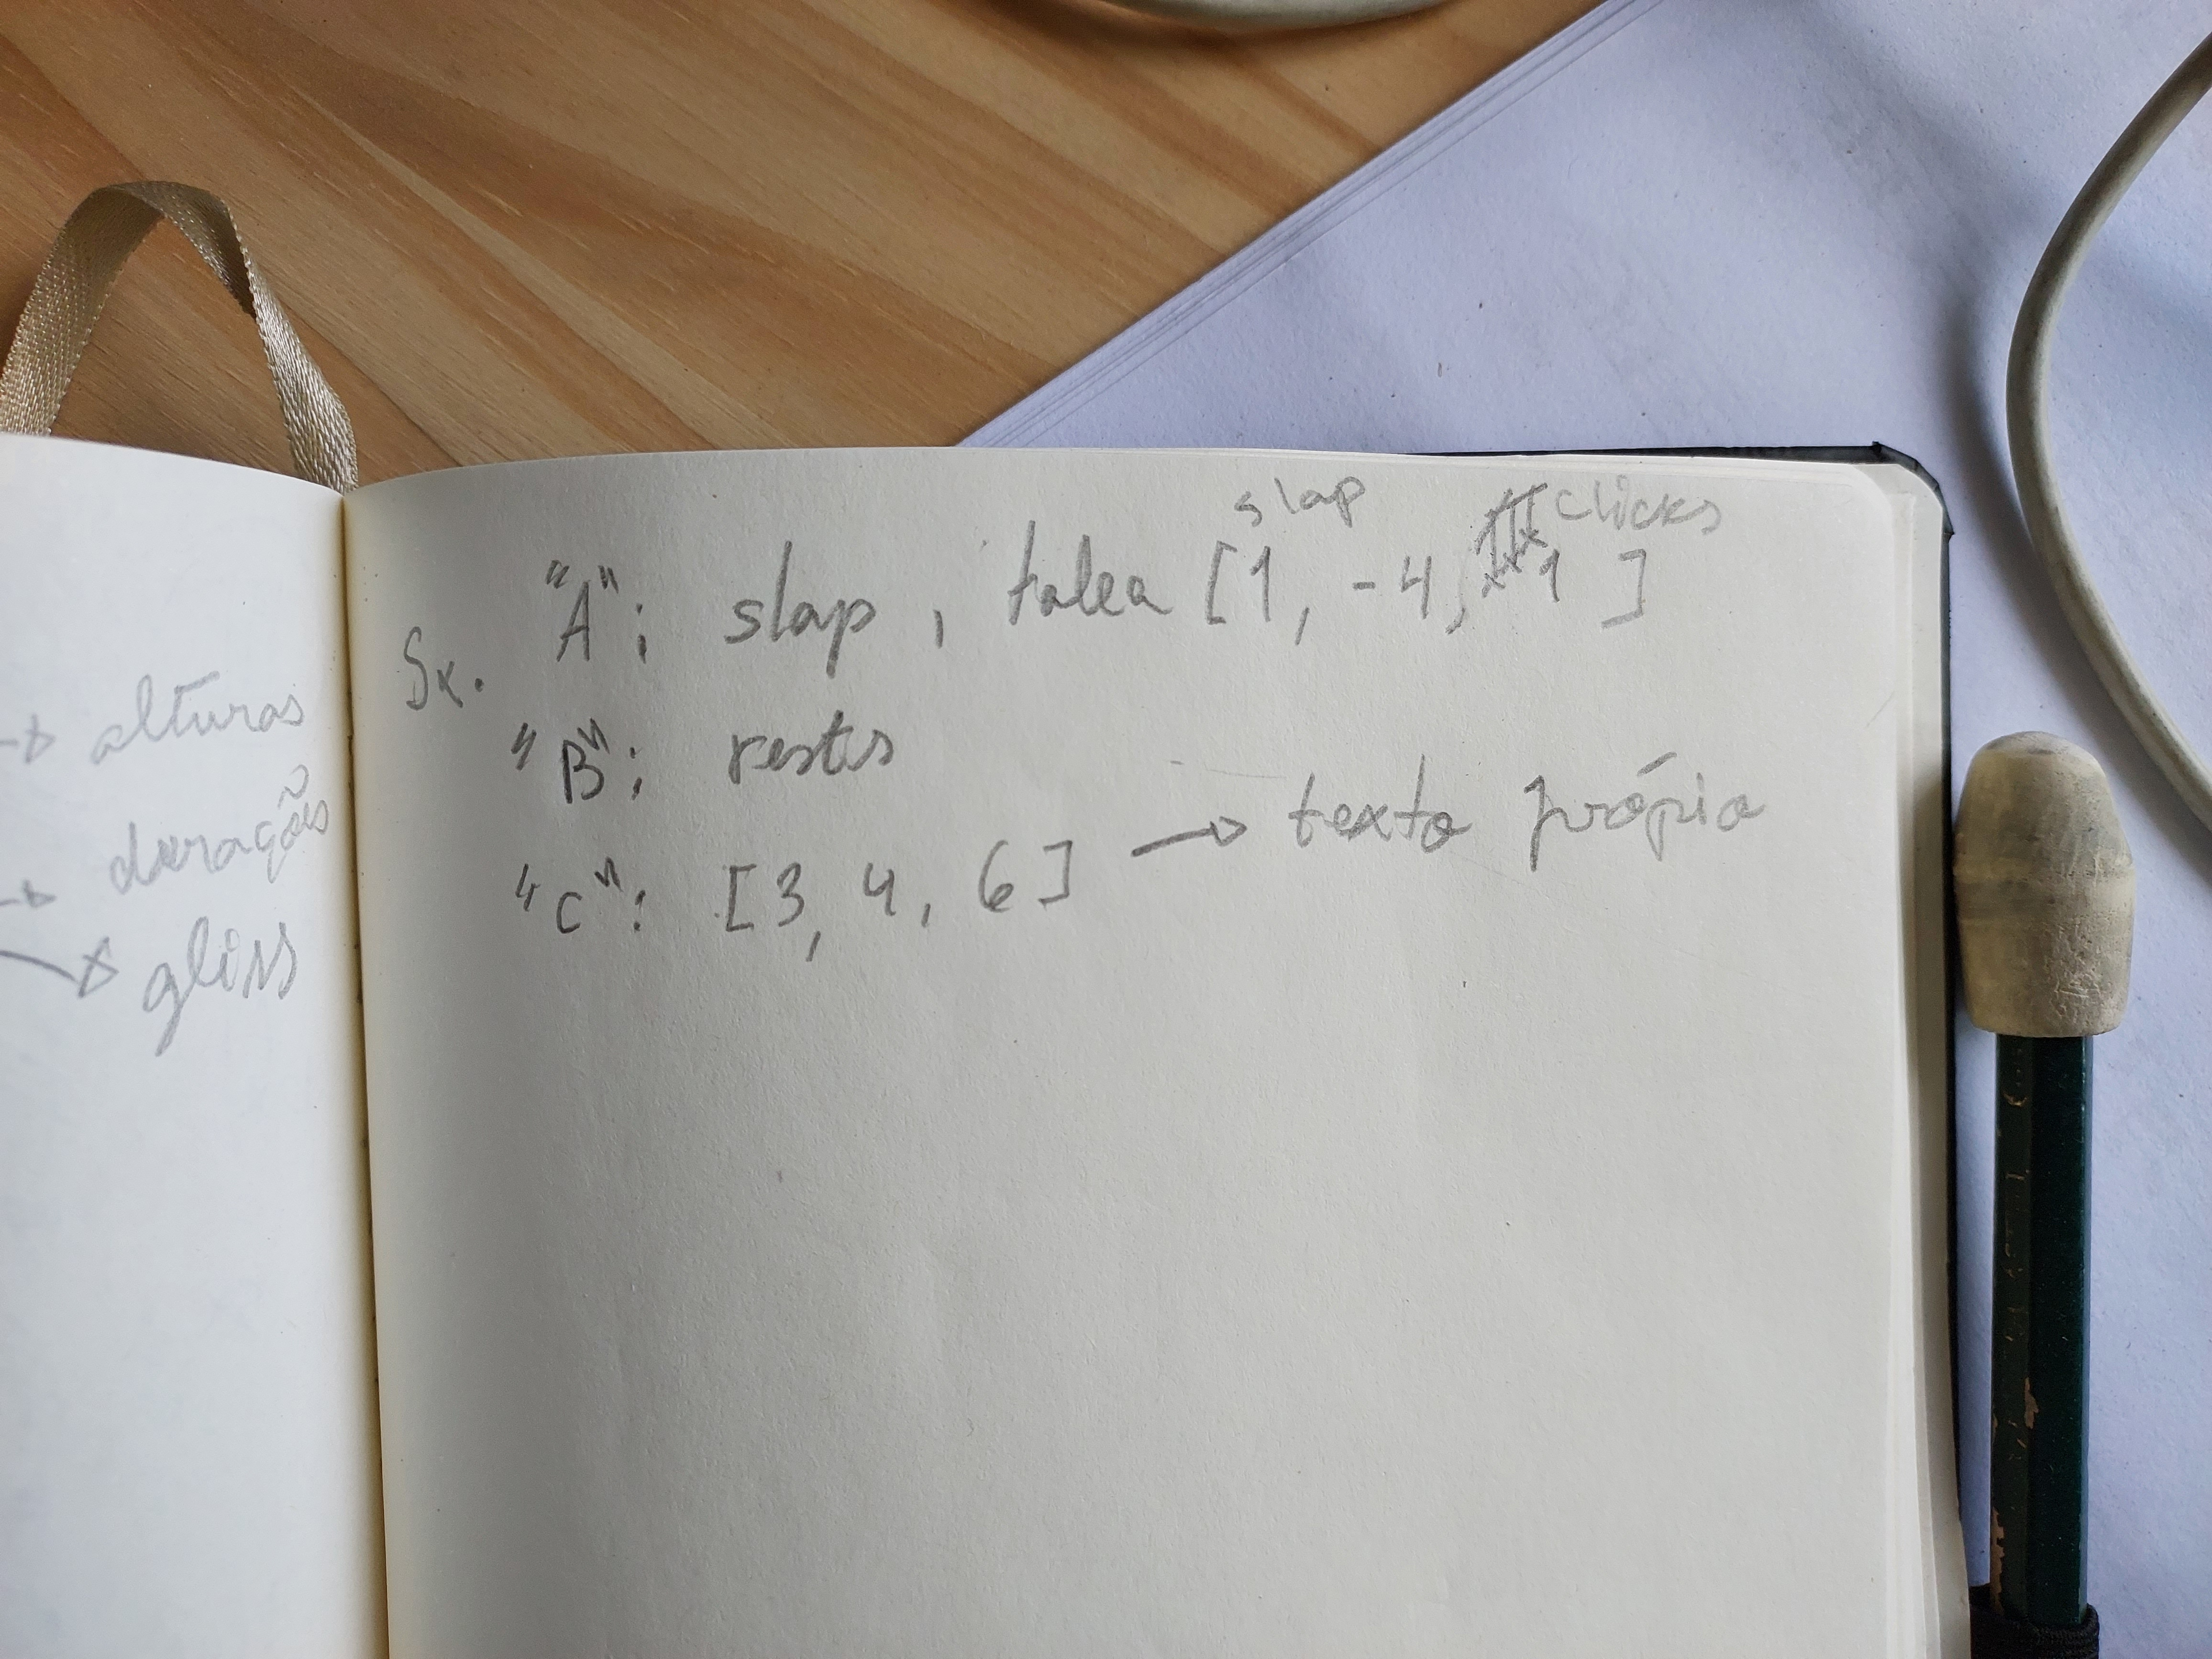
\includegraphics[width=10cm]{images/20230104_085636.jpg}
\end{center}

Embora esteja produzindo bastante (abaixo detalho algumas etapas do processo), não acredito que consigo finalizar esses 3 fragmentos até dia 14. Estou pensando em trabalhar na reescritura deste primeiro como maneira de gerar os outros dois. Por exemplo, aproveitar a mesma estrutura com outro percurso harmônico, ou com outro modo de leitura (inserindo mais pausas na leitura p. ex.), ou mudando para notação tradicional.

O trabalho até então envolve uma série de atividades que acho interessante mencionar:
\subsection*{Escrita do texto poético já pensado como estrutura temporal}
\label{sec:orgcc94063}

Estou trabalhando a partir do texto. Tento pensar o material musical como se fosse a leitura de um texto poético. 

O trecho abaixo se refere ao fragmento A. Para a apresentação abaixo (\textbf{diferente da partitura} \footnote{: Na partitura, o texto \sout{tachado} se refere à leitura mental (não falado).}), usei a seguinte notação:

normal = uma nota para cada sílaba

\sout{tachado} = pausa (leitura mental sem tocar)

\uline{sublinhado} = notas que se extendem por várias sílabas

\n

\textbf{Piccolo:}

Palavra \sout{salta, salta, voa}

atirada contra a água \sout{leve, leve, leve}

$\backslash$

salta, salta, voa

\uline{palavra} a - \uline{tirada}

pousa sobre as nuvens

pa - \uline{lavra} con - \uline{tra a água}

$\backslash$

mer - \uline{gulha cada vez mais} fundo

cada \uline{vez mais alto}

$\backslash$

a \uline{palavra seduz} a \uline{língua e escorre}

\sout{e escorre}, \uline{e escorre, e escorre}

\uline{cada vez mais sonhada}


$\backslash$


\textbf{Cello:} (retrógrado)

a \uline{palavra seduz} a \uline{língua e escorre}

\sout{e escorre}, \uline{e escorre, e escorre}

\uline{cada vez mais sonhada}

$\backslash$

mer - \uline{gulha cada vez mais} fundo

cada \uline{vez mais alto}

$\backslash$

salta, salta, voa

\uline{palavra} a - \uline{tirada}

pousa sobre as nuvens

pa - \uline{lavra} con - \uline{tra a água}

$\backslash$

Palavra \sout{salta, salta, voa}

atirada contra a água \sout{leve, leve, leve}

\subsubsection*{Funciona?}
\label{sec:org10708bc}
Faltou dizer na pré-composição 1 que se trata de leitura mental, o texto não será ouvido. Uso o texto tachado na partitura para indicar isso (falta fazer as notas de performance onde isso deve ficar claro).

Assim, a ideia é esta leitura associada (musical/textual) que apresenta grande flexibilidade em relação ao resultado, e ao mesmo tempo, um detalhamento em outro nível.

Márcio, não entendi se teu apontamento sobre esta técnica se referia ao caso específico do que apresentei, ou a técnica em si. O que apresentei, realmente não funcionaria muito bem porque estava aproveitando um texto e não tinha pensado o ritmo a partir do texto (as combinações texto/notas se davam por acaso). Agora, escrevi o texto e pensei os ritmos para ele, num processo parecido com o de musicar uma letra. O perfil melódico também derivou do texto.

Irá "funcionar" assim como "funcionou" na peça \href{https://www.youtube.com/watch?v=StGfpgi3p10}{As vozes das páginas}, embora não tenha certeza sobre o quanto funcionou naquela ocasião, ou melhor, não tenha certeza sobre o quanto esse funcionamento é interessante.

\subsection*{Códigos}
\label{sec:org579ff6d}
Tenho utilizado (pro bem e pro mal) o seguinte processo: Escrevo um programa em python (usando \href{https://abjad.github.io/}{abjad} e minha própria biblioteca \href{https://github.com/DaviRaubach/muda}{muda}) que gera uma partitura que é compilada pelo \href{https://lilypond.org/}{LilyPond} para gerar o pdf.
Devo subir o código da peça em breve para poder compartilhar com vocês.

\subsection*{Notação}
\label{sec:orgcb170b3}
Às vezes, um simples problema de notação demora a ser resolvido neste processo. Alterar uma articulação pode significar escrever uma função que selecione aquela nota numa lista de notas para modificá-la. Como a ideia não é trabalhar como se estivesse num programa gráfico, as funções tem que ser "espertas" e não voltadas a um único detalhe da partitura (embora isso aconteça algumas vezes).

O principal problema de notação neste caso é quanto a esta relação com o texto. Tenho escrito uma voz invisível na qual escrevo uma régua com o ritmo escrito da leitura do texto. Escrevo o ritmo sobre esta régua pensando na relação que terá com o texto (mais sílabas para uma única nota, ou pausa, etc.). Além disso, também precisei ocultar outras coisas da partitura e às vezes elas precisam reaparecer.

Optei por escrever cabeça de nota de semínima para notas associadas a uma única sílaba e cabeça de nota de mínima para notas associadas com mais sílabas.

\subsection*{Outras alturas}
\label{sec:org54a7eb0}
O percurso de alturas desse primeiro fragmento para o Piccolo é o seguinte:

\begin{verbatim}
1) multifônico 1 modulado (filtrado para extensão do piccolo)
sorted pitches: [18, 19, 21.5, 22, 23, 23.5, 24, 24.5, 25, 27, 30, 31]
used pitches: [23, 31, 25, 23, 21.5, 25, 24, 23, 21.5, 24, 18, 24, 23,
	       31, 23, 24, 21.5, 23, 24, 25]

2)multifônico 1 modulado + multifônico 2 (filtrado para extensão do piccolo)
sorted pitches: [18, 23, 23.5, 25, 30, 31]
used pitches: [25, 23.5, 23, 18, 30, 25, 23.5, 25, 23, 23.5, 18, 31, 18]

3) multifônico 2 modulado (filtrado para extensão do piccolo)
sorted pitches: [16, 17, 18, 19, 20, 20.5, 21, 22, 23, 23.5, 25, 26,
		 27, 28, 29, 30]
used pitches: [16, 23.5, 30, 19, 21, 16, 27]

4) multifônico 3 modulado (filtrado para extensão do piccolo)
sorted pitches: [16, 18, 19, 20, 20.5, 21, 22.5, 23.5, 24, 25.5, 26,
		 27, 27.5, 28, 29, 30, 31]
used pitches: [16, 22.5]
\end{verbatim}

Posso apresentar partitura destas alturas se alguém quiser.

\subsection*{Contágios}
\label{sec:org4ff4172}
O principal contágio é o uso do multifônico como gerador de alturas (Charles Neimog). Preciso encontrar outro contágio para explorar.


\section*{Partitura}
\label{sec:orgd7b159b}

Na partitura que estou enviando estão escritos apenas piccolo e cello. Falta pensar dinâmicas e articulações. Falta acertar o violão (notas superagudas com slide) e o sax (multifônicos dos quais derivam as alturas.

\begin{center}
\includegraphics[width=.9\linewidth]{omcwb_score.pdf}
\end{center}

\begin{center}
\includegraphics[width=.9\linewidth]{omcwb_scorep2.pdf}
\end{center}
\end{document}